\documentclass{article}
\usepackage{graphicx} % Required for inserting images
\documentclass{article}
\usepackage[utf8]{inputenc}
\usepackage{amsmath}
\usepackage{amssymb}
\usepackage{authblk}
\usepackage{setspace}
\usepackage[margin=1.25in]{geometry}
\usepackage{graphicx}
\graphicspath{ {./figures/} }
\usepackage{subcaption}
\usepackage{amsmath}
\usepackage{lineno}
\usepackage{hyperref}
\usepackage{comment}
\usepackage{lipsum}

\usepackage[style=nejm, 
citestyle=numeric-comp,
sorting=none]{biblatex}
\addbibresource{PartIIIProjectTemplate.bib}


\title{Variable change}
\author{PRABHODA C S}
\date{December 2024}

\begin{document}

\maketitle

\section{Introduction}  \label{Section 1}
Silvio \cite{Salvio_2022} and especially \cite{Pradisi_2022}, give us for the potential

\begin{equation}
    U(\omega) = \frac{1}{4 c'} \left[ \frac{M_{p}^{2}}{4} \text{sinh}(\text{X}(\omega)) - \beta  \right]^2
\end{equation}
where
\begin{equation}
    \text{X}(\omega) = \sqrt{\frac{2}{3}} \frac{\omega}{M_{p}} + \text{tanh}^{-1} \left(\frac{4 \beta}{\sqrt{M_{p}^{4}+16 \beta^2}} \right)
\end{equation}

Differentiating $U(\omega)$ and setting it equal to zero gives us that 

\begin{equation}
    \omega_{min} = \sqrt{\frac{2}{3}} M_p \left[ \text{sinh}^{-1}\left(\frac{4\beta}{M_{p}^{2}}\right) - \text{tanh}^{-1}\left(\frac{4\beta}{\sqrt{M_{p}^{4} + 16\beta^2}}\right) \right]
\end{equation}

Inserting $\text{ArcSinh(x)} = \ln(x + \sqrt{x^2 + 1})$ and $\text{ArcTanh(x)} = \frac{1}{2} \ln\left(\frac{1+x}{1-x}\right)$, gives us $\omega_{min} = 0$ always.
\\
Barker \cite{barker2024poincaregaugetheoryconformal} gives us potential

\begin{equation}
    U(\varphi) = \frac{\mu^2 \phi_{0}^{4}}{2} \left[ \frac{\sigma}{2} + \sqrt{\nu - \frac{\sigma^2}{4}} \text{sinh}\left( \text{X}(\varphi) \right)  \right]
\end{equation}
where
\begin{equation}
    \text{X}(\varphi) =  \frac{\varphi}{\phi_0 \sqrt{\nu - \frac{\sigma^2}{4}}} - \frac{c}{\phi_0 \sqrt{\nu - \frac{\sigma^2}{4}}}
\end{equation}

\section{Translating Variables}
We know that, $[\beta] = [M_{p}^{2}]$  and $[c'] = 0$ from \cite{Pradisi_2022}. If we want $\varphi = \omega$ (it can't be $\varphi = f(\omega)$ as that would ruin the $(\partial\varphi)^2$ term in Lagrangian), we are forced to make the substitutions that make dimensional sense:

\begin{align}
    \phi_0 &= \sqrt{\frac{3}{2}} M_p \label{eq:A} \\
    \mu &= \frac{1}{6 \sqrt{2 c'}} \label{eq:B} \\
    \sigma &= -\frac{8 \beta}{M_{p}^{2}} \label{eq:C} \\
    \nu &= 1 + \frac{16 \beta^2}{M_{p}^{4}} \label{eq:D} \\
    c  &= -\sqrt{\frac{3}{2}} M_{p} \text{tanh}^{-1} \left(\frac{4 \beta}{\sqrt{M_{p}^{4}+16 \beta^2}} \right) \label{eq:E}
\end{align}

Now, $[\phi_0] = [c] = [M_p]$ and the rest, $[\mu] = [\sigma] = [\nu] = 0$, to be fair, we can include a term $g^{-1}$ in front of the sinh term in $\text{X}(\omega)$, s.t., $[g] = 0$, the resulting eqns are:

\begin{align}
    \phi_0 &= g \sqrt{\frac{3}{2}} M_p \label{eq:A} \\
    \mu &= g^{-1} \frac{1}{6 \sqrt{2 c'}} \label{eq:B} \\
    \sigma &= - g^{-1} \frac{8 \beta}{M_{p}^{2}} \label{eq:C} \\
    \nu &= g^{-2} \left( 1 + \frac{16 \beta^2}{M_{p}^{4}} \right) \label{eq:D} \\
    c  &= -\sqrt{\frac{3}{2}} M_{p} \text{tanh}^{-1} \left(\frac{4 \beta}{\sqrt{M_{p}^{4}+16 \beta^2}} \right) \label{eq:E}
\end{align}

We can see that in \ref{eq:A}, the field $\varphi$ has no dependence on any parameter/is not free, but is fixed by the Planck mass (in Planck units, it is 1.225).

What we can see from equations \ref{eq:A} to \ref{eq:E}, is that $\phi_0 \propto M_p$, with the constant $g$ dictating what fraction of $M_p$,  $\phi_0$ is. $\mu$ is fixed by the strength of coupling of the $\mathcal{R'}^2$ term ($c'$) in the \cite{Pradisi_2022} paper. $c$ is now no longer free and based on the results from \ref{Section 1}, we see that the minima of the potential must now always stay at $\phi_{min} = 0$.

Below is a plot of the aligned graphs with $M_p = 1$ and the values of the parameters upon translation labelled. $g = \sqrt{\frac{1}{3}}$ so that $\phi_0 < M_p$ also.

\begin{figure}[h!]
    \centering
    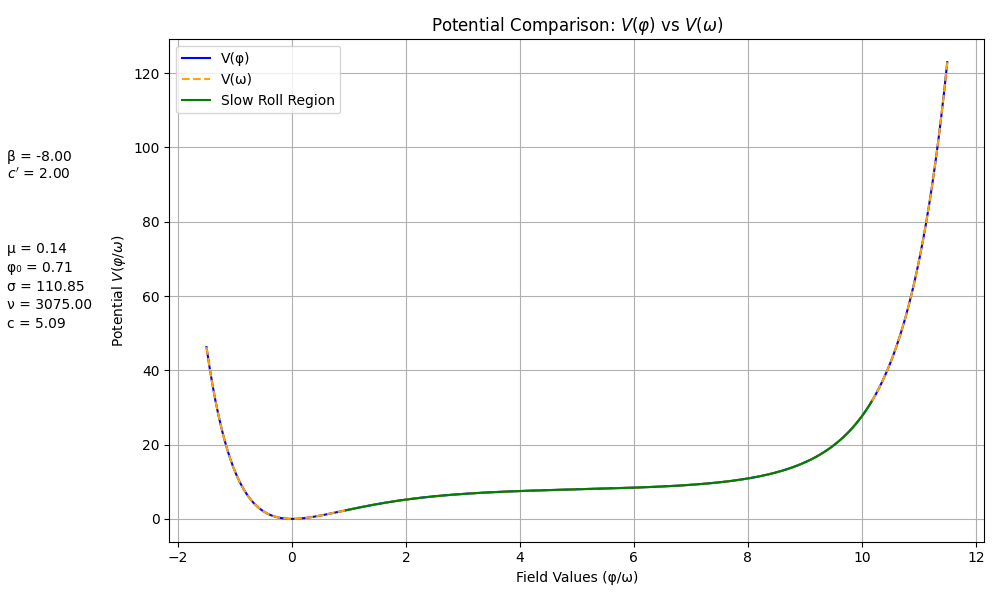
\includegraphics[width=1\textwidth]{Comparing Silvio - Barker.png}
    \caption{Aligned graphs with parameter values on the side}
    \label{Aligned Potential}
\end{figure}

For this value of $\beta$, we get $N = 73.582$ as the number of e-folds.


\newpage
\printbibliography

\end{document}
